%==================================================================================================
%   LUKES THESIS TEMPLATE 1.2
%   -------------------------
%   This template is based upon the offcial IMM PhD Thesis template, it is enhanced with a number
%   of new features and a number of errors have fixed. This template is intended to be complied to
%   PDF using PDFLATEX and is tested using the MiKTeX 2.9 LaTeX distribution.
%   It is based on the official DTU-IMM Thesis template by Finn Kuno Christensen in 2009.
%   Small bugfixes by Kasper Laursen in 2012 and 2013.
%   -------------------------
%   Last Updated: 2012-09-19
%   Contact: lthhe@imm.dtu.dk
%==================================================================================================
%
%==================================================================================================
% DOCUMENT SETUP
%==================================================================================================
\documentclass[10pt,twoside]{book}                  %Official DTU-IMM Thesis document setup
%
%Set to 'print' for printed version, use 'net' for online version
\def\thesisversion{print}
%
%==================================================================================================
% PACKAGES
%==================================================================================================
\usepackage{LukeThesis}                             %Import Thesis base style
%input{PhDMacros}                                   %Thesis specific macros
%
%==================================================================================================
% THESIS PROPERTIES (Modifiy these fields with your details)
%==================================================================================================
\def\thesisauthor{Luke Herbert}                     %Author
\def\thesistitle{Something something}               %Title
\def\thesishandin{01-January}                       %Submission date (Day-Month}
\def\thesisdegree{PhD}                              %Degree ('B.Eng', 'B.Sc.', 'M.Sc.' or 'PhD')
\def\thesisyear{2013}                               %Submission year
\def\thesisnumber{????}                             %DTU-IMM Serial number (do not include year)
\def\thesisISSN{0000-0000}                          %ISSN number
\def\thesiskeywords{Keywords are, comma separated}  %PDF keywords
\derivethesisprops                                  %Derive dependent properties
%
%==================================================================================================
% SECTION NUMBERING SETUP
%==================================================================================================
\setcounter{tocdepth}{2}                            %2 adds sections up to subsections
\setcounter{secnumdepth}{3}                         %Subsubsections get a number when this is 3
%
%==================================================================================================
% THESIS STRUCTURE  (Modifiy to include more chapters etc)
%==================================================================================================
\begin{document}
%------------------------
%Pre-frontmatter material
%------------------------
\prefrontmatter
%--------------------
%Frontmatter material
%--------------------
\frontmatter
\pagenumbering{roman}                               %Set frontmatter numbering style
\chapter{Summary (English)}

The goal of the thesis is to provide a method which infers the existence of physical co-location based on Bluetooth RSSI measurements. We gather two types of data through the use of mobile phones, which then we merge in a single set. We use the resulting set to analyse three algorithms: artificial neural networks, logistic regression and Naive Bayes. We vary the parameters of the algorithms and the features used and we compare the results. We look at how well the algorithms can infer co-location, as well as how computationally expensive they are. We finish this paper by recommending the combination of algorithm and feature that had the best results.                                       %English summary of Thesis
\markboth{}{}                                       %Set headings (left)(right)
\chapter{Summary (Danish)}
\begin{otherlanguage}{danish}

Målet for denne afhandling er at ...

\end{otherlanguage}                                   %Danish summary of Thesis
\markboth{}{}                                       %Set headings (left)(right)
\chapter{Preface}

This thesis was prepared at the department of Applied Mathematics and Computer Science at the Technical University of Denmark in fulfilment of the
requirements for acquiring an M.Sc. in Computer Science and Engineering.

%==================================================================================================
% SIGNATURE AREA
%==================================================================================================
\vspace{20mm}
\begin{center}
    \hspace{20mm} Lyngby, \thesishandin-\thesisyear
    \vspace{5mm}
    \newline
  %Update signature image file in line below
    
\includegraphics[scale=0.5]{figures/SignatureDummy}
\end{center}
\begin{flushright}
    \thesisauthor
\end{flushright}
% % % EOF % % %                                     %Preface
\markboth{}{}                                       %Set headings (left)(right)
\chapter{Acknowledgements}

I would like to thank my....

                            %Acknowledgements
\markboth{}{}                                       %Set headings (left)(right)
%------------------
% Table of contents
%------------------
\newpage\mbox{}\newpage
\chaptermark{Contents}
\pdfbookmark{\contentsname}{toc}
\renewcommand{\sectionmark}[1]{\markright{#1}}
\sectionmark{Contents}
\addtolength{\parskip}{-\baselineskip}
\tableofcontents
\addtolength{\parskip}{\baselineskip}
\renewcommand{\sectionmark}[1]{\markright{\thesection\ #1}}
%-------------
% Main content
%-------------
\mainmatter
\chapter{Introduction}

\section{Motivation}

Epidemiology \cite{human_sex}, personal health issues \cite{Madan}, group discovery \cite{5591535}, human mobility \cite{Sun2011929,sevtsuk}, efficient team creation \cite{ECTA, Pentland}, the analysis of academic success \cite{academics}, network theory \cite{networks}, also Fig. \ref{pic:dynamicsf2f}, and psychological research \cite{Rachuri}; all of the above have begun making use of the same notion, one that is difficult to quantify \cite{quant, Wilson}: social connections and social interactions between individuals. And although co-location does not necessarily mean physical social interaction, it is a requirement for it. \cite{Eagle08092009}.

\begin{figure}[h]
	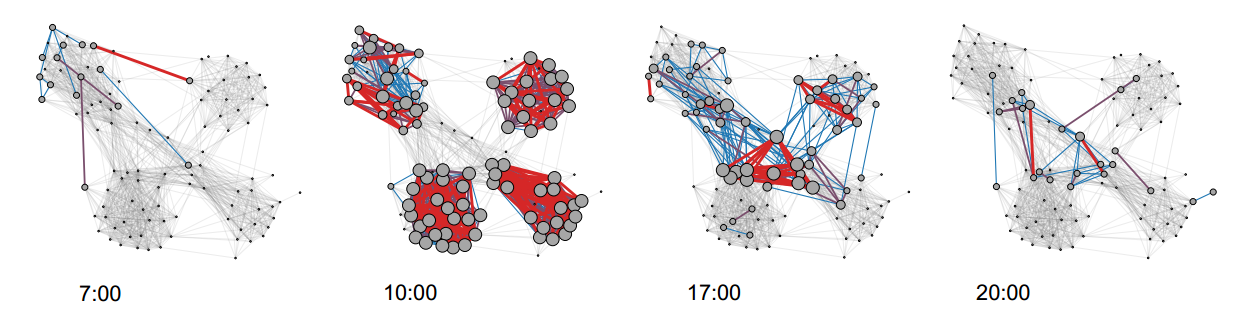
\includegraphics[scale=0.35]{figures/dynamicsf2f.png}
	\caption{Face-to-face interactions over a day for college students. Blue means a low, and red a high frequency of interactions. Image from \protect\cite{Stopczynski}}.
	\label{pic:dynamicsf2f}

\end{figure} 

There are a number of approaches to determining co-location: self-reported data, a more traditional approach, which is prone to cognitive bias, social desirability bias and halo error \cite{Wuchty08092009,gonyea}. A more recent approach involves the use of data provided by modern means of communication, namely mobile phones. This data can come from both the actual phone, in the form of GPS locations or bluetooth readings \cite{Stopczynski}, as well as from the phone company itself in the form of anonymous cell tower records \cite{Onnela01052007, hovel}. This has the advantage of being applicable almost anywhere, because of the high percentage of mobile phone penetration (95.5\% estimated by the International Telecommunication Union in May 2014). 
However, there are approaches that yield better results, but come with financial, environmental or other types of additional cost: RFID tags \cite{catt}, audio-video recordings \cite{audiovideo}, on-body sensors \cite{onbody} and wifi signals \cite{wifi}, just to name a few. 
 
 
\section{Objective}

Given a bluetooth RSSI between two phones, the purpose of this paper is to indicate a method which reliably and accurately determines the existence of pairwise co-location between the people carrying the two phones.

Reliability refers to the fact that multiple tries with the same input, and constant settings ( same machine learning algorithm, same parameters and same training data), will always yield exactly the same result. While accuracy refers to the precision of the algorithm during cross-validation testing, or how close to 100\% it is. 
 
This inference is achieved by applying and analysing multiple machine learning algorithms on a data set consisting of two main parts:
\begin{itemize}
  \item Data automatically recorded by the SensibleDTU data collector app \cite{Stopczynski}
  \item Ground truth data obtained by the test subjects by interacting with the FriendFinder app
\end{itemize}

For each machine learning algorithm the parameter configuration which yields the best results will be chosen, followed by a comparison between the best configurations for each algorithm.      

\section{Scope and limitations}

The paper analyses the data obtained from three test subjects. Each subject has been given the same phone model, Samsung Galaxy Nexus.

While considerable testing has been done with regards to the algorithm parameters, the machine learning algorithms list is by no means exhaustive. There are three main algorithms: Naive Bayes, Neural Networks, and Recursive learning, and an explanation on why a fourth, Hidden Markov Model, is unsuitable for this type of data. 

When analysing data, we only look at the bluetooth RSSI value, and data derived directly while measuring it. For example, given that measurements are taken every five minutes, we at some point look at the length of an uninterrupted string of measurements, or at the measurements taken before and after (if possible) a specific measurement. GPS traces, phone records, infrared sensors, or facebook/email information are not taken into consideration.

\section{Thesis Outline}

The thesis begins with this introduction, which gives an overview of the general theme of the project. The objectives, scope and limitations and thesis outline are all self-defining. 

It continues with a section which describes the data acquisition process and the methodology used to obtain the data from the SensibleDTU database. The section also describes the FriendFinder app, as well as its implementation.

Next, the machine learning algorithms are presented. For each algorithm a theoretical overview is given. The implementation details are discussed, followed by the results obtained by applying it to the data. At the end of this chapter, we do a comparative analysis between the algorithms, followed by the last section, the conclusions, where we will give the final results and recommandations.
                                  %Chapter 1
%\chapter{Data acquisition}

The data used in the paper has been gathered over the course of three months, starting in early March and ending in late May. The data has been obtained with the help of three student volunteers. Each volunteer carried a phone, provided by the SensibleDTU project, the same project this thesis is a part of \cite{sensibledtu, Stopczynski}. The phones are Samsung Galaxy Nexus \cite{nexus} and are running the Android operating system \cite{android}. 

Each phone came with two apps. The first recorded regularly a multitude of information, such as Bluetooth RSSI, GPS traces, battery usage and cell tower information, and is a part of the SensibleDTU project \cite{Stopczynski}, while the second allowed the volunteers to manually name the person they are in physical proximity with, and was developed during this thesis. The second app provided the ground-truth information.

This gave rise to two types of data. First, a continuous stream of regular measurements from the first app, and punctual messages from the second app. Below we will go into more detail about how exactly the two types of data look, how are they gathered and finally, how the two are combined to create a unitary set which serves as a basis for the machine learning algorithms.

\section{FriendFinder app}

\subsection{App overview and implementation}

As the app, FriendFinder, is made for the Android operating system, it is implemented using Java for Android \cite{jandroid}. It has a Google App Engine backend \cite{googleapp}. Fig \ref{pic:ff_prtscr} shows the main screen of the app. 

\begin{figure}[h]
	\begin{center}
		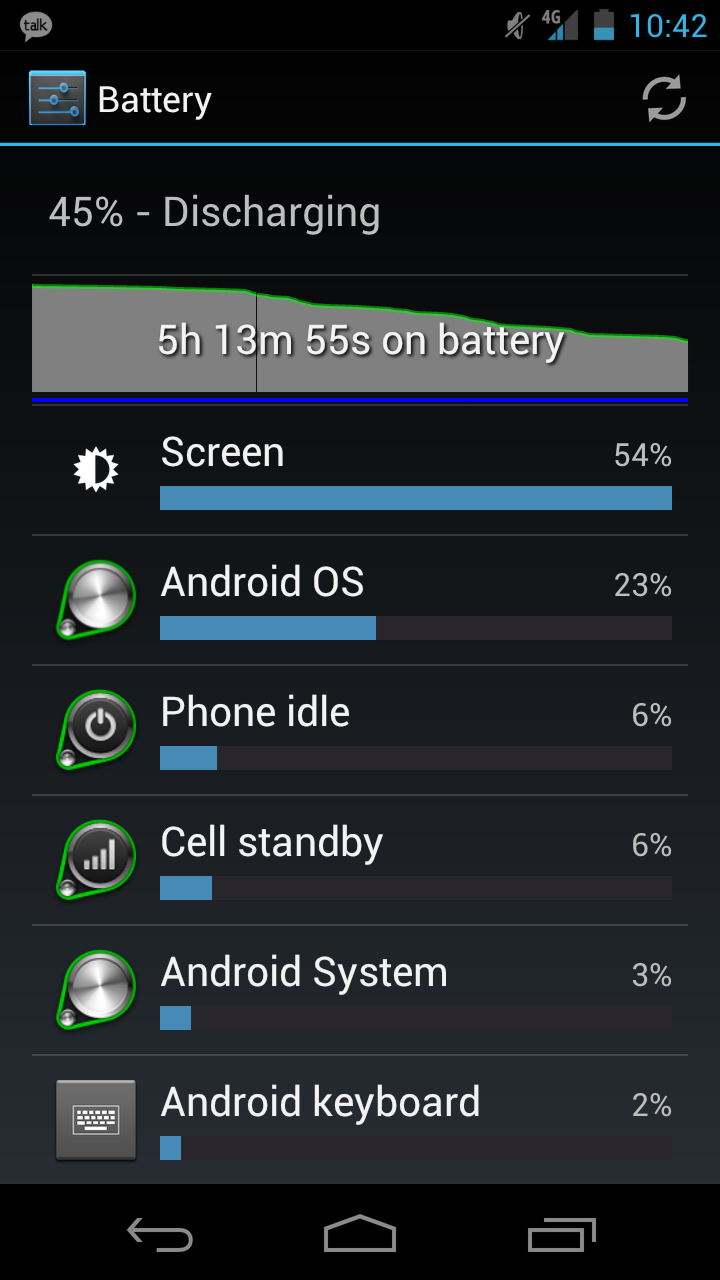
\includegraphics[scale=0.2]{figures/galaxy-nexus-battery.png}
	\end{center}
	
	\caption{FriendFinder app}.
	\label{pic:ff_prtscr}

\end{figure} 

FriendFinder is implemented using a client server architecture, where the clients are the apps installed on the phone, and the server is the Google App Engine. Fig \ref{pic:clientserver} shows an overview of this particular architecture. In this case, the FriendFinder app (in the role of the client) makes a \textit{save data} request to the Google App Engine (the server). The server in turn responds with the result of the operation, either a \textit{succes} or \textit{failure} message.  

\begin{figure}[h]
	\begin{center}
		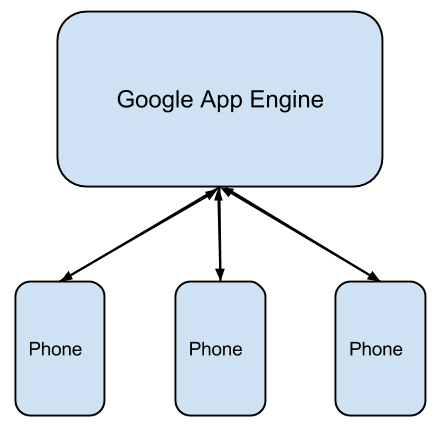
\includegraphics[scale=0.5]{figures/SC_Arch.png}
	\end{center}
	
	\caption{Client Server Architecture used by the FriendFinder app}.
	\label{pic:clientserver}

\end{figure} 

The app contains a single screen (the one showed in Fig \ref{pic:ff_prtscr}), which corresponds to the main activity. Activities are the main building blocks of an Android app, and they are used both to interact with the user, as well as provide additional functionalities \cite{activity}. On the main screen there are buttons for each volunteer. Once one of the volunteers is in physical proximity with another volunteer (as perceived by either one), they both press the button corresponding to each other. A confirmation message is displayed, as can be seen in Fig. \ref{pic:ff_conf}.

\begin{figure}[h]
	\begin{center}
		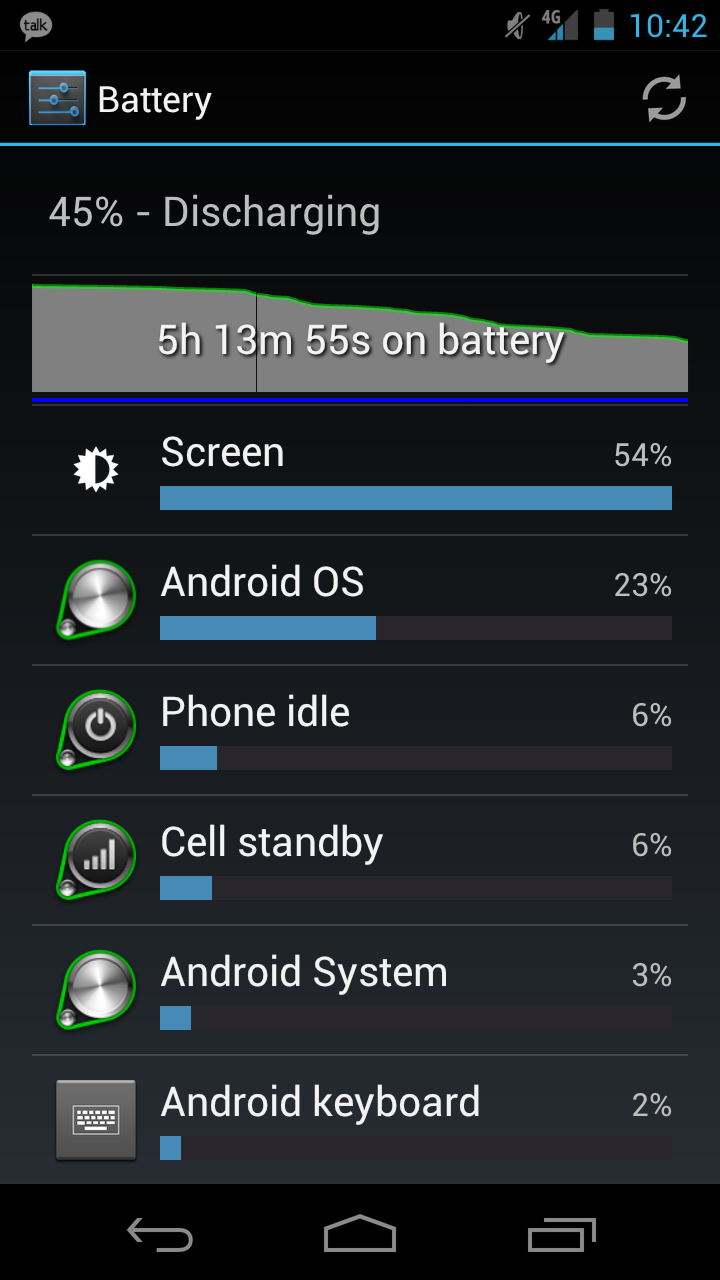
\includegraphics[scale=0.2]{figures/galaxy-nexus-battery.png}
	\end{center}
	
	\caption{Confirmation message on the FriendFinder app}.
	\label{pic:ff_conf}

\end{figure}

For the data to reach the database on the Google App Engine, an internet connection is required. However, the app can also function off-line, by saving all the data locally, and sending it to the on-line database as soon as an internet connection is established. It does this by using an IntentService \cite{intentservice}, which has two main functions:

\begin{itemize}
  \item A first function is to store the data locally, until an internet connection is established.
  \item the second, and most important, is to check periodically for an internet connections. Once an internet connection has been established, all the data is sent to the Google App Engine. The app checks every one minute for internet access. This allows for a relatively fast updating of the database, while at the same time keeping the resource use at a level that does not impede the normal functioning of the phone.
\end{itemize}

The data is stored locally in RAM of the phone (the volatile memory). This is made possible by the relatively small size of the data being saved ( the names of the two people involved, and an ID object that also serves as a timestamp) and the memory capacity of the phone ( approximately 700 MB of RAM). However, this has the disadvantage of being vulnerable to the phone turning off due to lack of battery. The volunteers have been made aware of this fact. 

Once the internet connection is established, the actual sending of the data is a simple matter, done with the help of the Google App Engine API. One thing to mention here is that each data entry is sent individually. If at any point, a \textit{save data} request is met by a \textit{failure} answer, the request is repeated until the \textit{success} message is received. In case of \textit{failure}, subsequent attempts have a one second delay between them. This is done to ensure that the app does not impede the overall functionality of the phone.



\subsection{Data}

Once a button with the name of a person is pressed, the data that is saved on the phone, and eventually sent and saved on the online database has the following format:

\begin{verbatim}
{ID, owner, target}
\end{verbatim}

\begin{description}
  \item[ID] It has a double role. First, the ID is a unique identifier, used for differentiating between multiple entries, as well as for various database operations. This field is required by the Google App Engine. Secondly, the ID also plays the role of the timestamp, used in future computations. While there are valid concerns that the ID might not be unique, due to two people pressing the button at the same time, the fact that the timestamp also includes the millisecond, and the fact that there are only three participants in the project results in an extremely low probability of identical timestamps. Obviously, the timestamp corresponds to the moment the button was pressed, and not the moment the data was sent to the database.  
  \item[owner] This field refers to the owner of the phone, which indicates the person that has made the observation.
  \item[target] This field names the person that has been observed by the owner.
\end{description}

Fig. \ref{pic:dataviewer} shows an example of how the data looks, with the caveat that the \textit{friend} field in the image corresponds to the \textit{target} field in the description above. The saved data was accessed and retrieved by API calls to the Google App Engine.  

\begin{figure}[h]
	\begin{center}
		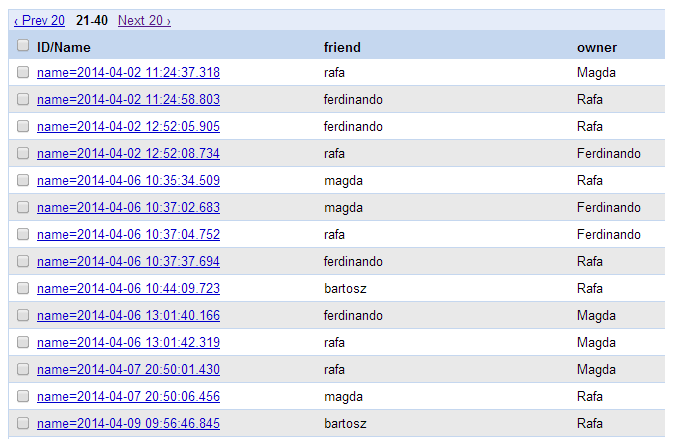
\includegraphics[scale=0.8]{figures/datastore.png}
	\end{center}
	
	\caption{Saved entries for the FriendFinder app}.
	\label{pic:dataviewer}

\end{figure}


\section{SensibleDTU data}

 The second type of data comes from the SensibleDTU data collector app. Based on \cite{Stopczynski,sensibledtu}, we will give a short description of the project, with an emphasis on data collection. We will then focus on the actual data, its form, and how it was collected. 

\subsection{Project overview}
 
 SensibleDTU is the implementation of a large scale study aimed at observing the various interchanges that take place between humans from a social and communications point of view. It aims to collect data on a large group of individuals, most of them students at DTU (Danish Technical University). The collected data consists of, among others, social relations and the networks that form as a result, geographical locations, and, of special interest to this thesis, face-to-face interactions. It does this by using a wide variety of sources, such as questionnaires, the wireless internet on campus, and mobile sensing through smartphones that were handed out to participants. A part of the data gathered through this last method is used in this thesis.
 
The smartphone data gathering is done by using a data collection app, based on the Funf framework \cite{funf}. This data is saved locally on the phone, and it is sent to a secure database server when the app detects the presence of an internet connection. Due to its sensitive nature, great care has been taken to ensure the privacy, security and anonymity of the saved data. Having said that, the three volunteers that participated in the data gathering for this thesis have agreed to the de-anonymization of their Bluetooth information, as it was required in order to merge the two sets of data gathered. 
 
 
\subsection{Data} 

The Bluetooth data is obtained periodically by the data collection app using the Bluetooth probe. Each phone performs a Bluetooth scan every five minutes. The scan lasts 30 seconds. While the 30 second scan lasts, the app saves all Bluetooth devices (that are discoverable) in its proximity, the time at which the scan has been made, as well as the RSSI \cite{vedran}. The data is stored on the phone from where it eventually reaches the secure database server, from where it can be downloaded. 

In order for the data to be used, it first needs to be \textit{cleaned}, as it contains additional meta-data ( fields used by the database for internal accounting), and devices that are not relevant to the thesis. The end result has the following format:

\begin{verbatim}
{time, owner, target,signal_strength}
\end{verbatim}
 
 The above tuple has almost the same format as the one resulted from the FriendFinder app, with the addition of the new field, signal strength. At a first glance, one might think that the two sets of data can be easily combined. However, due to differences in the time when data gathering takes place, de-synchronization and the human factor, obtaining a single data set from the two is not a trivial matter. The following section goes into more detail regarding this issue.
 
\section{Data merger}                                 %Chapter 2
\appendix
\chapter{Appendix}

\section{Examples of data formats from SensibleDTU app}

The data displayed here is not real, but the format is accurate. 

\begin{lstlisting}
{"timestamp_added": 1326129999, "name": "edu.mit.media.funf.probe.builtin.BluetoothProbe", "timestamp": 1384118284, "probe": "edu_mit_media_funf_probe_builtin_BluetoothProbe", "uuid": "1b3f4fe8-fffb-445c-bf52-5277ba67159-v0.3.2.4-0.5", "user": "d82fd5ca764f93bc38de04987ff13f", "device": "97e4ac7b-5aad-4190-83ac-b1f5ab40e487", "device_bt_mac": "E4:B0:21:E2:BF:10", "_id": "b21f904210a5a2b2cf408fa1cd2e34db_d82fa764f93bc3887ff13f_138297", "data": {"TIMESTAMP": 1394118297, "PROBE": "edu.mit.media.funf.probe.builtin.BluetoothProbe", "DEVICES": [{"android_bluetooth_device_extra_DEVICE": {"mAddress": "6e96626852eeaa41a2922780aff31767c6e842f34b20acffa49f6cb03"}, "android_bluetooth_device_extra_CLASS": {"mClass": 1573132}, "android_bluetooth_device_extra_RSSI": -73, "android_bluetooth_device_extra_NAME": "278450befb3d42372af5556577d0d9d"}, {"android_bluetooth_device_extra_DEVICE": {"mAddress": "f0ce0583a6c2f6743ccd8ed3a6f27b14c280c0c0cc4b1ed478"}, "android_bluetooth_device_extra_CLASS": {"mClass": 3801356}, "android_bluetooth_device_extra_RSSI": -78, "android_bluetooth_device_extra_NAME": "3db16e2f261af1c8c88ae88b0a9d546e2ab3e7329179"}]}, "sensible_token": "8e1754d8090059f8c4910d8897", "device_id": "bd955a5204e7e08de0eae2d9002d77e2"}
\end{lstlisting}

\begin{lstlisting}
"1b768078564005168dda562defa5b","1d7786b4b125656f74","ce4ad2c34123553c3b72b60e4eab19971456f5f391ed7","-82","2014-03-19 10:57:43"
"1b768f942564005168dda562defa5b","1d7786b4b121679bb9b5800eb46f74","9835c86c172aa3398564112455b42f54009a1ce37478d905f998d3f6c7","-73","2014-03-19 10:57:43"
"1b768f9412450516332defa5b","1d7786b4b13d04679bb9b58643b46f74","818dd0f1afd862c52b112262709c641b1995567ba28c3c20e","-57","2014-03-19 10:57:43"
"1b768f942564005168dda562defa5b","1d778234b13d04679bb9b5800eb46f74","8547c45679a561f8cbfff70de8572f161206ea06ce380a973","-88","2014-03-19 10:57:43"
"1b768f9425641234dda562defa5b","1d7786b412379bb9b5800eb46f74","818dd0f1afd862c52b8bdd65c37562709c641b19977c4ba1315057ba28c3c20e","-55","2014-03-19 11:02:43"
"1b768f942564005168444efa5b","1d7786b412323679bb9b5800eb46f74","ce4ad2c3477aef48ca1431004c023c3b72b60e4eab199712391ed7","-90","2014-03-19 11:02:43"
\end{lstlisting}


\section{The SensibleDTU data collection app}

Fig~\ref{pic:sensapp} shows the SensibleDTU data collection app login screen. 

\begin{figure}[h]
	\begin{center}
		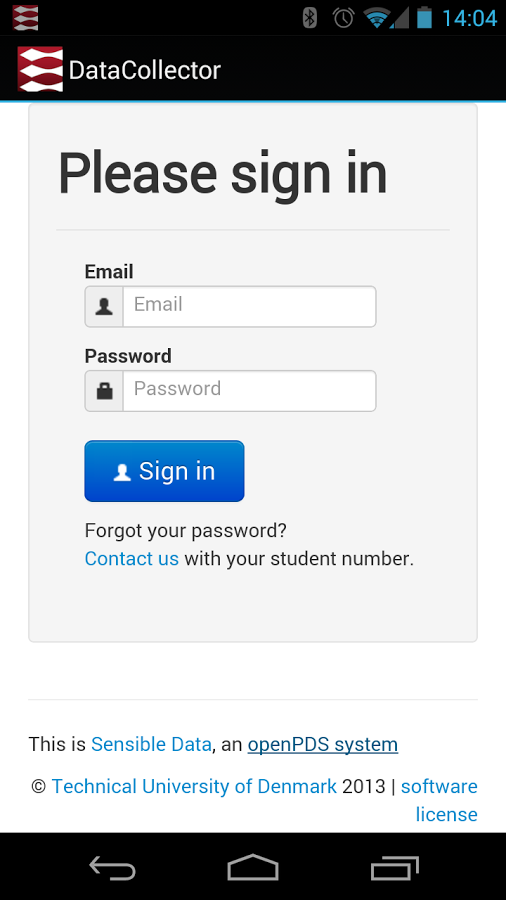
\includegraphics[scale=0.4]{figures/sensibleapp.png}
	\end{center}
	
	\caption{SensibleDTU data collection app.}
	\label{pic:sensapp}

\end{figure}                                 %Appendix A
%-----------
% Backmatter
%-----------
\backmatter
\chaptermark{Bibliography}
\renewcommand{\sectionmark}[1]{\markright{#1}}
\sectionmark{Bibliography}
\addcontentsline{toc}{chapter}{Bibliography}        %Force addition of Bibliography to TOC
\bibliographystyle{alpha}                           %Use alpha codes for references
\bibliography{References}                           %Bibliography file called
\end{document}
% % % EOF % % %